\documentclass[journal, a4paper]{IEEEtran}
%\author{Huidong Lin}
% some very useful LaTeX packages include:

%\usepackage{cite}      % Written by Donald Arseneau
                        % V1.6 and later of IEEEtran pre-defines the format
                        % of the cite.sty package \cite{} output to follow
                        % that of IEEE. Loading the cite package will
                        % result in citation numbers being automatically
                        % sorted and properly "ranged". i.e.,
                        % [1], [9], [2], [7], [5], [6]
                        % (without using cite.sty)
                        % will become:
                        % [1], [2], [5]--[7], [9] (using cite.sty)
                        % cite.sty's \cite will automatically add leading
                        % space, if needed. Use cite.sty's noadjust option
                        % (cite.sty V3.8 and later) if you want to turn this
                        % off. cite.sty is already installed on most LaTeX
                        % systems. The latest version can be obtained at:
                        % http://www.ctan.org/tex-archive/macros/latex/contrib/supported/cite/

\usepackage{graphicx}   % Written by David Carlisle and Sebastian Rahtz
                        % Required if you want graphics, photos, etc.
                        % graphicx.sty is already installed on most LaTeX
                        % systems. The latest version and documentation can
                        % be obtained at:
                        % http://www.ctan.org/tex-archive/macros/latex/required/graphics/
                        % Another good source of documentation is "Using
                        % Imported Graphics in LaTeX2e" by Keith Reckdahl
                        % which can be found as esplatex.ps and epslatex.pdf
                        % at: http://www.ctan.org/tex-archive/info/

%\usepackage{psfrag}    % Written by Craig Barratt, Michael C. Grant,
                        % and David Carlisle
                        % This package allows you to substitute LaTeX
                        % commands for text in imported EPS graphic files.
                        % In this way, LaTeX symbols can be placed into
                        % graphics that have been generated by other
                        % applications. You must use latex->dvips->ps2pdf
                        % workflow (not direct pdf output from pdflatex) if
                        % you wish to use this capability because it works
                        % via some PostScript tricks. Alternatively, the
                        % graphics could be processed as separate files via
                        % psfrag and dvips, then converted to PDF for
                        % inclusion in the main file which uses pdflatex.
                        % Docs are in "The PSfrag System" by Michael C. Grant
                        % and David Carlisle. There is also some information
                        % about using psfrag in "Using Imported Graphics in
                        % LaTeX2e" by Keith Reckdahl which documents the
                        % graphicx package (see above). The psfrag package
                        % and documentation can be obtained at:
                        % http://www.ctan.org/tex-archive/macros/latex/contrib/supported/psfrag/

%\usepackage{subfigure} % Written by Steven Douglas Cochran
                        % This package makes it easy to put subfigures
                        % in your figures. i.e., "figure 1a and 1b"
                        % Docs are in "Using Imported Graphics in LaTeX2e"
                        % by Keith Reckdahl which also documents the graphicx
                        % package (see above). subfigure.sty is already
                        % installed on most LaTeX systems. The latest version
                        % and documentation can be obtained at:
                        % http://www.ctan.org/tex-archive/macros/latex/contrib/supported/subfigure/

\usepackage{url}        % Written by Donald Arseneau
                        % Provides better support for handling and breaking
                        % URLs. url.sty is already installed on most LaTeX
                        % systems. The latest version can be obtained at:
                        % http://www.ctan.org/tex-archive/macros/latex/contrib/other/misc/
                        % Read the url.sty source comments for usage information.

%\usepackage{stfloats}  % Written by Sigitas Tolusis
                        % Gives LaTeX2e the ability to do double column
                        % floats at the bottom of the page as well as the top.
                        % (e.g., "\begin{figure*}[!b]" is not normally
                        % possible in LaTeX2e). This is an invasive package
                        % which rewrites many portions of the LaTeX2e output
                        % routines. It may not work with other packages that
                        % modify the LaTeX2e output routine and/or with other
                        % versions of LaTeX. The latest version and
                        % documentation can be obtained at:
                        % http://www.ctan.org/tex-archive/macros/latex/contrib/supported/sttools/
                        % Documentation is contained in the stfloats.sty
                        % comments as well as in the presfull.pdf file.
                        % Do not use the stfloats baselinefloat ability as
                        % IEEE does not allow \baselineskip to stretch.
                        % Authors submitting work to the IEEE should note
                        % that IEEE rarely uses double column equations and
                        % that authors should try to avoid such use.
                        % Do not be tempted to use the cuted.sty or
                        % midfloat.sty package (by the same author) as IEEE
                        % does not format its papers in such ways.

\usepackage{amsmath}    % From the American Mathematical Society
                        % A popular package that provides many helpful commands
                        % for dealing with mathematics. Note that the AMSmath
                        % package sets \interdisplaylinepenalty to 10000 thus
                        % preventing page breaks from occurring within multiline
                        % equations. Use:
%\interdisplaylinepenalty=2500
                        % after loading amsmath to restore such page breaks
                        % as IEEEtran.cls normally does. amsmath.sty is already
                        % installed on most LaTeX systems. The latest version
                        % and documentation can be obtained at:
                        % http://www.ctan.org/tex-archive/macros/latex/required/amslatex/math/
\usepackage[outputdir=build]{minted}
\usepackage{amssymb}
\usepackage{amsmath}
\usepackage[hidelinks]{hyperref} 

\newcommand{\argmin}{\arg\!\min}

% Other popular packages for formatting tables and equations include:

%\usepackage{array}
% Frank Mittelbach's and David Carlisle's array.sty which improves the
% LaTeX2e array and tabular environments to provide better appearances and
% additional user controls. array.sty is already installed on most systems.
% The latest version and documentation can be obtained at:
% http://www.ctan.org/tex-archive/macros/latex/required/tools/

% V1.6 of IEEEtran contains the IEEEeqnarray family of commands that can
% be used to generate multiline equations as well as matrices, tables, etc.

% Also of notable interest:
% Scott Pakin's eqparbox package for creating (automatically sized) equal
% width boxes. Available:
% http://www.ctan.org/tex-archive/macros/latex/contrib/supported/eqparbox/

% *** Do not adjust lengths that control margins, column widths, etc. ***
% *** Do not use packages that alter fonts (such as pslatex).         ***
% There should be no need to do such things with IEEEtran.cls V1.6 and later.


% Your document starts here!
\begin{document}
\begin{titlepage}

\newcommand{\HRule}{\rule{\linewidth}{0.5mm}} % Defines a new command for the horizontal lines, change thickness here

\center % Center everything on the page
 %----------------------------------------------------------------------------------------
%	LOGO SECTION
%----------------------------------------------------------------------------------------

~\\[1cm]
\includegraphics{/home/oidiotlin/Pictures/SCUT-full-logo.png}\\[2cm] % Include a department/university logo - this will require the graphicx package

%----------------------------------------------------------------------------------------
%	TITLE SECTION
%----------------------------------------------------------------------------------------

\HRule \\[1cm]
{ \huge \bfseries The Experiment Report of \textit{Machine Learning} }\\[0.6cm] % Title of your document
\HRule \\[2cm]
%----------------------------------------------------------------------------------------
%	HEADING SECTIONS
%----------------------------------------------------------------------------------------


\textsc{\LARGE \textbf{School:} School of Software Engineering}\\[1cm]
\textsc{\LARGE \textbf{Subject:} Software Engineering}\\[2cm] 

 
%----------------------------------------------------------------------------------------
%	AUTHOR SECTION
%----------------------------------------------------------------------------------------

\begin{minipage}{0.4\textwidth}
\begin{flushleft} \large
\emph{Author:}\\
Huidong Lin % Your name
\end{flushleft}
\end{minipage}
~
\begin{minipage}{0.4\textwidth}
\begin{flushright} \large
\emph{Supervisor:} \\
Qingyao Wu % Supervisor's Name
\end{flushright}
\end{minipage}\\[2cm]
~
\begin{minipage}{0.4\textwidth}
\begin{flushleft} \large
\emph{Student ID:}\\
201636665056
\end{flushleft}
\end{minipage}
~
\begin{minipage}{0.4\textwidth}
\begin{flushright} \large
\emph{Grade:} \\
Undergraduate
\end{flushright}
\end{minipage}\\[2cm]

% If you don't want a supervisor, uncomment the two lines below and remove the section above
%\Large \emph{Author:}\\
%John \textsc{Smith}\\[3cm] % Your name

%----------------------------------------------------------------------------------------
%	DATE SECTION
%----------------------------------------------------------------------------------------

{\large October 8, 2018}\\[2cm] % Date, change the \today to a set date if you want to be precise

 
%----------------------------------------------------------------------------------------

\vfill % Fill the rest of the page with whitespace

\end{titlepage}

% Define document title and author
	\title{Linear Regression: Closed-Form Solution and Stochastic Gradient Descent}
	\maketitle

% Write abstract here
\begin{abstract}
% The short abstract is intended to give the reader an overview of the experiment. It should be brief and to the point. 
    This experiment intends to use closed-form solution and stochastic gradient descent algorithm for regression problem.
\end{abstract}

% Each section begins with a \section{title} command
\section{Introduction}
	% \PARstart{}{} creates a tall first letter for this first paragraph
% \PARstart{T}{his} section introduces the problem to solved and leads the reader on to the main part. Detailed motivation is necessary. What's more, you can show your expected results and contributions.
    \PARstart{L}{inear} regression model is used widely in machine learning field. The most popular algorithms for solving the model parameters are closed-form solution and stochastic gradient descent (SGD). I reproduced these two algorithms and evaluated them on Housing dataset of LIBSVM Data\footnote{LIBSVM Data - Housing: \url{https://www.csie.ntu.edu.tw/~cjlin/libsvmtools/datasets/regression.html\#housing}}

% Main Part
\section{Methods and Theory}
% In this section, you are asked to give a complete introduction to the experiment. For instance, the chosen methods, the related theories, the related equations(loss function), the derivation process(taking the gradient) and so on.
\subsection{Linear Regression Model}

Given a data set $\{y_i, x_i^{(1)}, \ldots, x_i^{(m)}\}_{i=1}^n$ of $n$ statistical units, a linear regression model assumes that the relationship between the dependent variable $y$ and the $m$-vector of regressors $\mathbf{x}$ is linear, which can be represented as

\begin{equation}
    \begin{split}
        y_i & = \theta_1 x_i^{(1)} + \cdots + \theta_m x_i^{(m)} + b \\ 
            & = \mathbf{x}^\mathsf{T}\boldsymbol{\theta} + b \qquad\qquad\qquad\qquad i = 1,\ldots,n    
    \end{split}
\end{equation}

These $n$ equations are usually written in matrix notation as

\begin{equation}
    \mathbf{y} = X\boldsymbol{\theta} + \mathbf{b}
\end{equation}

\subsection{Loss Function}

Squared loss $\mathcal{L}(\boldsymbol{\theta}):\mathbb{R}^n\mapsto\mathbb{R}$ is used for measuring performance of the regression model.

\begin{equation}\label{eq:loss}
    \mathcal{L}(\boldsymbol{\theta}) = \frac{1}{2}\sum^n_{i=1} (y_i-\boldsymbol\theta^{\mathsf{T}}\mathbf{x})^2
\end{equation}

\subsection{Closed-Form Solution}

According to \eqref{eq:loss}, it is supposed to find the best $\boldsymbol{\theta}$ to minimize the loss, which can be represented as

\begin{equation}\label{eq:closed-form}
    \begin{split}
        \boldsymbol{\theta}^{\ast} & = \argmin_{\boldsymbol{\theta}}\mathcal{L}(\boldsymbol{\theta}) \\
                                   & = \left(X^\mathsf{T}X\right)^{-1}X^\mathsf{T}\mathbf{y}
    \end{split}
\end{equation}

\subsection{Stochastic Gradient Descent}

In standard gradient descent algorithm

\begin{equation}\label{eq:gd}
    \begin{split}
        \boldsymbol\theta_t & \leftarrow \boldsymbol\theta_{t-1} - \eta\nabla_{\boldsymbol\theta_{t-1}}\mathcal{L}(\boldsymbol\theta_{t-1}) \\
                            & = \boldsymbol\theta_{t-1} - \frac{\eta}{n}\sum^{n}_{i=1}\nabla_{\boldsymbol\theta_{t-1}}\mathcal{L}_i(\boldsymbol\theta_{t-1})
    \end{split}
\end{equation}

In \eqref{eq:gd}, $\mathcal{L}_i$ is loss on $i$-th sample. Thus, the direction of gradient depends on the whole dataset. 

Stochastic gradient descent chooses only one of the dataset to calculate the gradient

\begin{equation}\label{eq:sgd}
    \boldsymbol\theta_t \leftarrow \boldsymbol\theta_{t-1} - \eta\nabla_{\boldsymbol\theta_{t-1}}\mathcal{L}_i(\boldsymbol\theta_{t-1})
\end{equation}

In \eqref{eq:sgd}, $i$ is the random chosen sample index. For vector details, the gradient can be written as

\begin{equation}\label{eq:gradient}   
    \frac{\partial\mathcal{L}(\boldsymbol\theta)}{\partial\boldsymbol\theta} = 
    \begin{bmatrix}
        \frac{\partial\mathcal{L}(\boldsymbol\theta)}{\partial\boldsymbol\theta_1} \\
        \frac{\partial\mathcal{L}(\boldsymbol\theta)}{\partial\boldsymbol\theta_2} \\
        \vdots \\
        \frac{\partial\mathcal{L}(\boldsymbol\theta)}{\partial\boldsymbol\theta_m}
    \end{bmatrix}
\end{equation}

For $L2$-loss, the gradient should be

\begin{equation}\label{eq:l2loss-gradient}
    \nabla_{\boldsymbol\theta}\mathcal{L}(\boldsymbol\theta) = X^{\mathsf{T}}(\mathbf{\hat{y}} - \mathbf{y}) = X^{\mathsf{T}}(X\boldsymbol\theta - \mathbf{y})
\end{equation}

\section{Experiments}
\subsection{Dataset}
% This section represents the related information of datasets, such as the content, the number of data, the training set, the validation set and so on.

    This dataset was taken from the StatLib library which is maintained at Carnegie Mellon University, concerning housing values in suburbs in Boston in 1978. It contains 506 independent samples, each of which includes a median value of owner-occupied homes in \$1000\textquotesingle s (predicting target) and 13 attributes(features) which are scaled in $[-1, 1]$.

\subsection{Implementation}
\subsubsection{Initialization}
    The dataset is split to validation set and training set with ratios $(20\%, 80\%)$ respectively. Both of the two algorithm use random normal distribution for parameter $\boldsymbol\theta$ initialization.
    
    $$\boldsymbol\theta \sim N(\mu=1, \sigma^2=1)$$
    
\subsubsection{Parameters}
\paragraph{Closed-Form Solution}
    There is no hyper parameter in closed-form solution.
\paragraph{Stochastic Gradient Descent}
    There are two hyper parameters in SGD algorithm as Table~\ref{tab:sgd-hyperparams} shown.
    \begin{table}[!hbt]
        \begin{center}
            \caption{Hyper Parameters of SGD}
            \label{tab:sgd-hyperparams}
            \begin{tabular}{l|l}
                \hline
                Parameters & Values \\
                \hline
                Number of epochs & $200$ \\
                Learning rate & $3\times 10^{-4}$ \\
                \hline
            \end{tabular}
        \end{center}
    \end{table}
    
\subsubsection{Results}
\paragraph{Closed-Form Solution}
    . Figure~\ref{fig:closed-form-prediction} shows prediction $\hat{y}$ and truth $y$ on validation set.
    
    \begin{table}[!hbt]
        \begin{center}
        \caption{Losses in Closed-Form Solution}
        \label{tab:closed-form-losses}
        \begin{tabular}{l|l|l}
            \hline
            Phase & Dataset & $L2$-Loss \\
            \hline
            Initialization & training & $556.68$ \\
            Trained & training & $23.72$ \\
            Trained & validtion & $27.20$ \\
            \hline
        \end{tabular}
        \end{center}
    \end{table}    
    
    \begin{figure}[!hbt]
        \begin{center}
        \caption{Prediction and Truth}
        \label{fig:closed-form-prediction}
        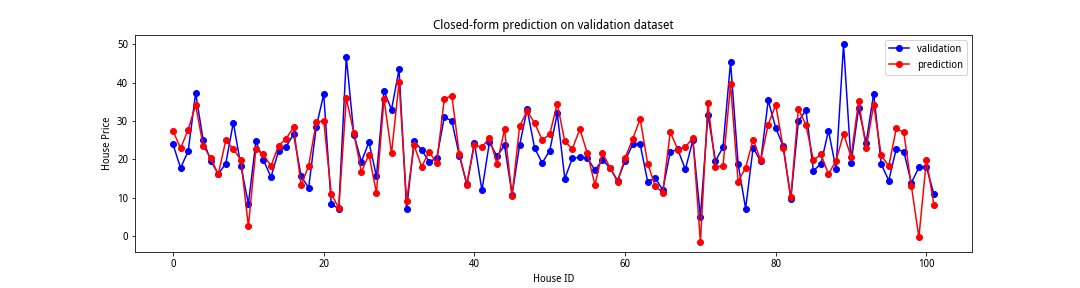
\includegraphics[width=\columnwidth]{../images/closed-form-prediction.png}
        \end{center}
    \end{figure}
    
\paragraph{Stochastic Gradient Descent}
    Table~\ref{tab:sgd-losses} shows varying losses on different phases in the experiment. Figure~\ref{fig:sgd-losses} shows varying losses on training and validation set during training process. Figure~\ref{fig:sgd-prediction} shows prediction $\hat{y}$ and truth $y$ on validation set.
    
    \begin{table}[!hbt]
        \begin{center}
        \caption{Losses in SGD}
        \label{tab:sgd-losses}
        \begin{tabular}{l|l|l}
            \hline
            Phase & Dataset & $L2$-Loss \\
            \hline
            Initialization & training & $727.42$ \\
            Trained & training & $26.50$ \\
            Trained & validtion & $29.19$ \\
            \hline
        \end{tabular}
        \end{center}
    \end{table}
    
    \begin{figure}[!hbt]
        \begin{center}
        \caption{Losses in SGD}
        \label{fig:sgd-losses}
        \includegraphics[width=\columnwidth]{../images/sgd-losses.png}
        \end{center}
    \end{figure}
    
    \begin{figure}[!hbt]
        \begin{center}
        \caption{Prediction and Truth}
        \label{fig:sgd-prediction}
        \includegraphics[width=\columnwidth]{../images/sgd-prediction.png}
        \end{center}
    \end{figure}

    The gradient descent is very smooth, which means that the descent process meets the requirements of this lab. In addition, the descent process of the loss of train and the loss of evaluation are similar, which means that the hyper-parameters chosen are suitable.

\section{Conclusion}
	Closed-Form Solution and Stochastic Gradient Descent both have great performance on chosen dataset in this experiment. On dataset with small scale, closed-form solution has better performance than SGD. However, closed-form can be extremely slow as dataset scale grows because of its $O(n^3)$ time complexity (calculation for inverse of $X$ matrix). Thus, SGD is widely used for minimizing $\mathcal{L}(\boldsymbol\theta)$ when large dataset is involved to avoid calculation explosion.


% Your document ends here!
\end{document}